\documentclass[10pt,letterpaper,subeqn]{beamer}
\setbeamertemplate{navigation symbols}{}
\usefonttheme{serif}
\usecolortheme{seahorse}



\usepackage[english]{babel}
\selectlanguage{english}
\usepackage{bm}
\usepackage{booktabs}
\usepackage{color}
\usepackage[update,prepend]{epstopdf}
\usepackage{framed}
\usepackage{fleqn}
\usepackage{graphics}
\usepackage{hyperref}
\usepackage[utf8]{inputenc}
\usepackage{setspace}
\usepackage{textcomp}
\usepackage{wrapfig}
\usepackage{multirow}
\usepackage{caption}
\usepackage{subcaption}
\usepackage{subfloat}
\setbeamertemplate{caption}[numbered]
\usepackage{wrapfig}
\usepackage{tikz}

\definecolor{cadmiumgreen}{rgb}{0.0, 0.42, 0.24}
\usetikzlibrary{trees}
\usetikzlibrary{decorations.markings}


%================================================================================
%== TITLE, NAMES, DATE
%================================================================================
\title{The Value of Season of Birth and Fertility Timing}

\author{Damian Clarke\inst{\dag} 
   \and Sonia Oreffice\inst{\ddag} 
   \and Climent Quintana-Domeque\inst{*}}

\institute{\inst{\dag}  University of Oxford
      \and \inst{\ddag} University of Surrey and IZA 
      \and \inst{*}     University of Oxford and IZA}

\date{June 2015}
%********************************************************************************
\begin{document}


\begin{frame}
\titlepage
\end{frame}

%********************************************************************************

\begin{frame}[label=sum]
\input{./tables/sumStatsnvss.tex}
\end{frame}

\begin{frame}[label=BQs]
\input{./tables/sumsinglenvss.tex}
\end{frame}


\begin{frame}[label=births]
\frametitle{Maternal Age at Birth: USA}
\begin{figure}[htpb!]
\begin{center}
  \centering
  \caption{Mother's Age at First Birth, 25-45 (NVSS)}
  \includegraphics[scale=0.6]{./../results/nvss/graphs/ageDescriptive.eps}
  \label{fig:NVSSbirths}
\end{center}
\end{figure}
\vspace{-5mm}
\end{frame}

\begin{frame}[label=births]
\frametitle{Maternal Age at Birth: USA}
\begin{figure}[htpb!]
\begin{center}
  \centering
  \caption{Difference in Births (\% Good Season - \% Bad Season)}
  \includegraphics[scale=0.6]{./../results/nvss/graphs/birthQdiff.eps}
  \label{fig:NVSSbirths}
\end{center}
\end{figure}
\vspace{-5mm}
\footnotesize{Note: `Young' refers to 25-39.  `Old' refers to 40-45.}
\end{frame}

\begin{frame}[label=births]
\frametitle{Maternal Age at Birth: USA}
\begin{figure}[htpb!]
\begin{center}
  \centering
  \caption{Difference in Births (\% Good Season - \% Bad Season)}
  \includegraphics[scale=0.6]{./../results/nvss/graphs/birthQdiff_4Ages.eps}
  \label{fig:NVSSbirthsAges}
\end{center}
\end{figure}
\vspace{-5mm}
\end{frame}

\begin{frame}[label=twins]
\frametitle{Twin Prevalance and Age}
\begin{figure}[htpb!]
\begin{center}
  \centering
  \caption{Proportion of Twins Born by Age}
  \includegraphics[scale=0.6]{./../results/nvss/graphs/twinPrevalence.eps}
  \label{fig:NVSSTwins}
\end{center}
\end{figure}
\vspace{-5mm}
\end{frame}


\begin{frame}[label=ART]
\frametitle{Assisted Reproductive Technology and Age}
\begin{figure}[htpb!]
\begin{center}
  \centering
  \caption{Proportion of Mothers Reporting any ART}
  \includegraphics[scale=0.6]{./../results/nvss/graphs/ART.eps}
  \label{fig:NVSSART}
\end{center}
\end{figure}
\vspace{-5mm}
\footnotesize{Notes: Questions on ART use are only included in 2012-2013 
birth certificate data.}
\end{frame}


\begin{frame}[label=QBw]
\frametitle{Birth Quality by Season}
\begin{figure}[htpb!]
\centering
\caption{Child quality: Birthweight (grams)}
\label{QBwt}
\includegraphics[scale=0.6]{../results/nvss/graphs/AllQuality_birthweight_.eps}
\end{figure}
\end{frame}

\begin{frame}[label=QBwEd]
\frametitle{Birth Quality by Season}
\begin{figure}[htpb!]
\centering
\caption{Child quality: Birthweight by Education}
\label{QBwtEd}
\includegraphics[scale=0.6]{../results/nvss/graphs/Quality_birthweight_.eps}
\end{figure}
\end{frame}

\begin{frame}[label=NVSSseason]
\frametitle{Season of Birth, Age and Education}
\begin{table}[htbp]\centering
\def\sym#1{\ifmmode^{#1}\else\(^{#1}\)\fi}
\caption{Birth Quarter and Age (NVSS 2005-2013)}
\scalebox{0.8}{
\begin{tabular}{l*{4}{c}}
\toprule
                    &\multicolumn{1}{c}{(1)}   &\multicolumn{1}{c}{(2)}   &\multicolumn{1}{c}{(3)}   &\multicolumn{1}{c}{(4)}   \\
                    & Good Season   & Good Season   & Good Season   & Good Season   \\
\midrule
Aged 25-39          &       0.019***&       0.019***&       0.020***&       0.006   \\
                    &     [0.001]   &     [0.001]   &     [0.002]   &     [0.005]   \\
College Educ        &               &               &       0.010***&      -0.005   \\
                    &               &               &     [0.001]   &     [0.005]   \\
College$\times$ Aged 25-39&               &               &               &       0.015***\\
                    &               &               &               &     [0.005]   \\
Constant            &       0.497***&       0.497***&       0.488***&       0.501***\\
                    &     [0.001]   &     [0.001]   &     [0.002]   &     [0.005]   \\
\midrule
R-squared           &        0.00   &        0.00   &        0.00   &        0.00   \\
Observations        &     4871628   &     4871628   &     3613920   &     3613920   \\
Year FE&&Y&Y&Y\\ \bottomrule
\multicolumn{5}{p{12cm}}{\begin{footnotesize}Sample consists of all
first born children of US-born, white, non-hispanic mothers
\end{footnotesize}}\end{tabular}}\end{table}

\end{frame}

\begin{frame}[label=NVSSseasonQ]
\frametitle{Season of Birth, Age and Education}
\input{./tables/quarterHeterogeneity.tex}
\end{frame}

\begin{frame}[label=NVSSseasonQ]
\frametitle{Season of Birth, Age and Education (Multinomial Logit)}
INSERT MULTINOMIAL LOGIT RESULTS ONCE MARGINS HAVE RUN.
\end{frame}


\begin{frame}
\frametitle{Conception and Births: YOUNG}
\begin{figure}
\hspace{6.0cm}{\footnotesize \textbf{Realized Season}} \vspace{4mm}\\
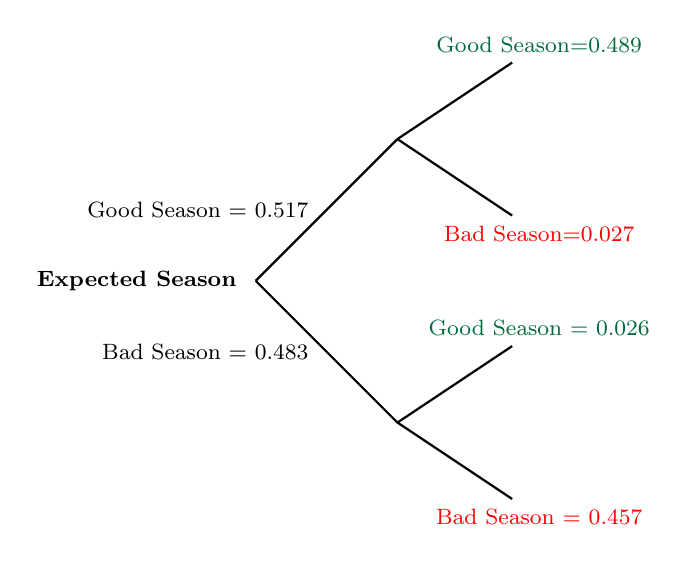
\begin{tikzpicture}[scale=0.6,thick,
    level/.style={level distance=3cm},
    level 2/.style={sibling distance=6cm},
    level 3/.style={sibling distance=4cm}
]
\coordinate
child[grow=right, level distance=0pt] {
        child  {
            child {
                node {{\footnotesize \textcolor{red}{Bad Season = 0.457}}}
                edge from parent 
            }
            child {
                node {{\footnotesize \textcolor{cadmiumgreen}{Good Season = 0.026}}}
                edge from parent
            }
            edge from parent
            node [left] {{\footnotesize Bad Season = 0.483 \ }}
        }
        child {
            child {
                node {{\footnotesize \textcolor{red}{Bad Season=0.027}}}
                edge from parent
            }
            child {
                node {{\footnotesize \textcolor{cadmiumgreen}{Good Season=0.489}}}
                edge from parent  
            }
            edge from parent 
            node [left] {{\footnotesize Good Season = 0.517 \ }}
        }
        node [left] {{\footnotesize \textbf{Expected Season\ \ }}}
    };
\end{tikzpicture}
\end{figure}
\end{frame}

\begin{frame}
\frametitle{Conception and Births: OLD}
\begin{figure}
\hspace{6.0cm}{\footnotesize \textbf{Realized Season}} \vspace{4mm}\\
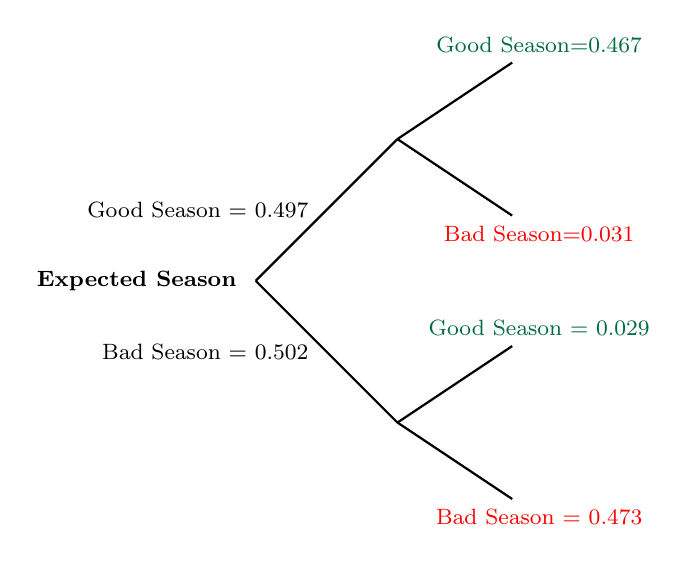
\begin{tikzpicture}[scale=0.6,thick,
    level/.style={level distance=3cm},
    level 2/.style={sibling distance=6cm},
    level 3/.style={sibling distance=4cm}
]
\coordinate
child[grow=right, level distance=0pt] {
        child  {
            child {
                node {{\footnotesize \textcolor{red}{Bad Season = 0.473}}}
                edge from parent 
            }
            child {
                node {{\footnotesize \textcolor{cadmiumgreen}{Good Season = 0.029}}}
                edge from parent
            }
            edge from parent
            node [left] {{\footnotesize Bad Season = 0.502 \ }}
        }
        child {
            child {
                node {{\footnotesize \textcolor{red}{Bad Season=0.031}}}
                edge from parent
            }
            child {
                node {{\footnotesize \textcolor{cadmiumgreen}{Good Season=0.467}}}
                edge from parent  
            }
            edge from parent 
            node [left] {{\footnotesize Good Season = 0.497 \ }}
        }
        node [left] {{\footnotesize \textbf{Expected Season\ \ }}}
    };
\end{tikzpicture}
\end{figure}
\end{frame}

\begin{frame}[label=EdInteract]
\frametitle{Season of Birth, Age and Education}
\input{./tables/NVSSBinaryEdInteract.tex}
\end{frame}

\begin{frame}[label=birthSeasonYoung34]
\frametitle{Season of Birth, Age and Education}
\input{./tables/NVSSBinaryYoung34.tex}
\end{frame}

\begin{frame}
\frametitle{First Birth Rates by Mother's Age: 35-39 vs. 40-44}
\begin{center}
\includegraphics[scale=0.3]{./tables/Figure_1.png}
\end{center}
\end{frame}

\begin{frame}
\frametitle{First Birth for Mother's Age 40-44 by Race and Ethnicity}
\begin{center}
\includegraphics[scale=0.3]{./tables/Figure_3.png}
\end{center}
\end{frame}



\begin{frame}[label=NVSSQuality]
\frametitle{Birth Quality}
\begin{table}[htbp]\centering
\def\sym#1{\ifmmode^{#1}\else\(^{#1}\)\fi}
\caption{Birth Quality by Age and Season (NVSS 2005-2013)}
\scalebox{0.68}{
\begin{tabular}{l*{7}{c}}
\toprule
                    &\multicolumn{1}{c}{(1)}   &\multicolumn{1}{c}{(2)}   &\multicolumn{1}{c}{(3)}   &\multicolumn{1}{c}{(4)}   &\multicolumn{1}{c}{(5)}   &\multicolumn{1}{c}{(6)}   &\multicolumn{1}{c}{(7)}   \\
                    &       APGAR   & Birthweight   &   Gestation   &         LBW   &   Premature   &        Twin   &        VLBW   \\
\midrule
Aged 25-39          &       0.043***&     130.718***&       0.598***&      -0.055***&      -0.064***&      -0.054***&      -0.010***\\
                    &     [0.004]   &     [2.581]   &     [0.011]   &     [0.001]   &     [0.001]   &     [0.001]   &     [0.000]   \\
Bad Season          &       0.002   &      -5.653   &      -0.011   &       0.004** &       0.002   &       0.001   &      -0.001*  \\
                    &     [0.005]   &     [3.585]   &     [0.015]   &     [0.002]   &     [0.002]   &     [0.001]   &     [0.001]   \\
Young$\times$ Bad S &      -0.005   &      -4.781   &      -0.014   &      -0.001   &       0.001   &       0.001   &       0.002***\\
                    &     [0.005]   &     [3.638]   &     [0.015]   &     [0.002]   &     [0.002]   &     [0.001]   &     [0.001]   \\
College Educ        &       0.045***&      77.112***&       0.181***&      -0.025***&      -0.021***&       0.010***&      -0.006***\\
                    &     [0.001]   &     [0.917]   &     [0.004]   &     [0.000]   &     [0.000]   &     [0.000]   &     [0.000]   \\
&&&&&&&\\
Constant            &       8.756***&    3121.397***&      38.034***&       0.150***&       0.194***&       1.075***&       0.028***\\
                    &     [0.004]   &     [2.775]   &     [0.012]   &     [0.001]   &     [0.001]   &     [0.001]   &     [0.001]   \\
\midrule
R-squared           &        0.00   &        0.00   &        0.00   &        0.00   &        0.00   &        0.00   &        0.00   \\
Observations        &     3551931   &     3603294   &     3610749   &     3613920   &     3613920   &     3613920   &     3613920   \\
\bottomrule
\multicolumn{8}{p{15cm}}{\begin{footnotesize}Sample consists of all
first born children of US-born, white, non-hispanic mothers
\end{footnotesize}}\end{tabular}}\end{table}

\end{frame}

\begin{frame}[label=NVSSQuality]
\frametitle{Birth Quality}
\input{./tables/qualityHeterogeneity.tex}
\end{frame}

\begin{frame}[label=NVSSQuality]
\frametitle{Birth Quality}
\input{./tables/QualityAllComb.tex}
\end{frame}

\begin{frame}[label=NVSSQuality]
\frametitle{Birth Quality}
\input{./tables/QAllYoung1.tex}
\end{frame}

\begin{frame}[label=NVSSQuality]
\frametitle{Birth Quality}
\input{./tables/QAllYoung0.tex}
\end{frame}


\begin{frame}[label=Spainseason]
\frametitle{Season of Birth, Age and Education (Spain)}
\input{./tables/spainBinary.tex}
\end{frame}

\begin{frame}[label=SpainQuality]
\frametitle{Birth Quality (Spain)}
\input{./tables/spainQualityEduc.tex}
\end{frame}

\begin{frame}[label=SpainQuality]
\frametitle{Birth Quality (Spain)}
\input{./tables/spainQualityGestFix.tex}
\end{frame}



\begin{frame}
\frametitle{Conception and Births: YOUNG (Spain)}
\begin{figure}
\hspace{6.0cm}{\footnotesize \textbf{Realized Season}} \vspace{4mm}\\
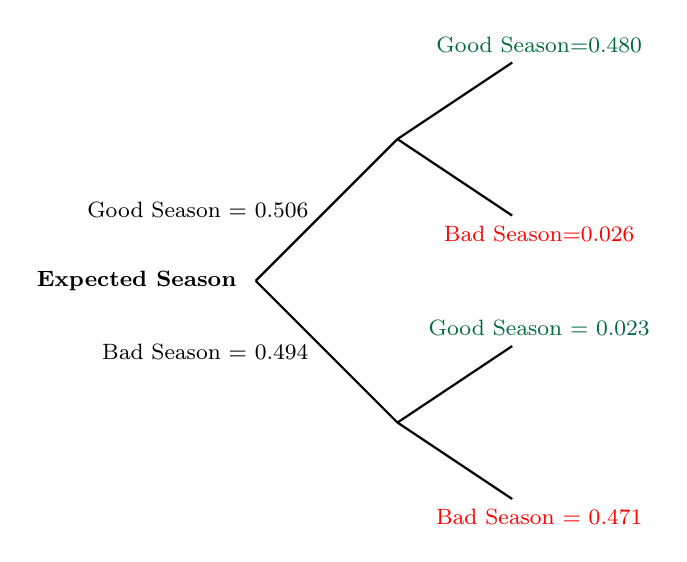
\begin{tikzpicture}[scale=0.6,thick,
    level/.style={level distance=3cm},
    level 2/.style={sibling distance=6cm},
    level 3/.style={sibling distance=4cm}
]
\coordinate
child[grow=right, level distance=0pt] {
        child  {
            child {
                node {{\footnotesize \textcolor{red}{Bad Season = 0.471}}}
                edge from parent 
            }
            child {
                node {{\footnotesize \textcolor{cadmiumgreen}{Good Season = 0.023}}}
                edge from parent
            }
            edge from parent
            node [left] {{\footnotesize Bad Season = 0.494 \ }}
        }
        child {
            child {
                node {{\footnotesize \textcolor{red}{Bad Season=0.026}}}
                edge from parent
            }
            child {
                node {{\footnotesize \textcolor{cadmiumgreen}{Good Season=0.480}}}
                edge from parent  
            }
            edge from parent 
            node [left] {{\footnotesize Good Season = 0.506 \ }}
        }
        node [left] {{\footnotesize \textbf{Expected Season\ \ }}}
    };
\end{tikzpicture}
\end{figure}
\end{frame}

\begin{frame}
\frametitle{Conception and Births: OLD (Spain)}
\begin{figure}
\hspace{6.0cm}{\footnotesize \textbf{Realized Season}} \vspace{4mm}\\
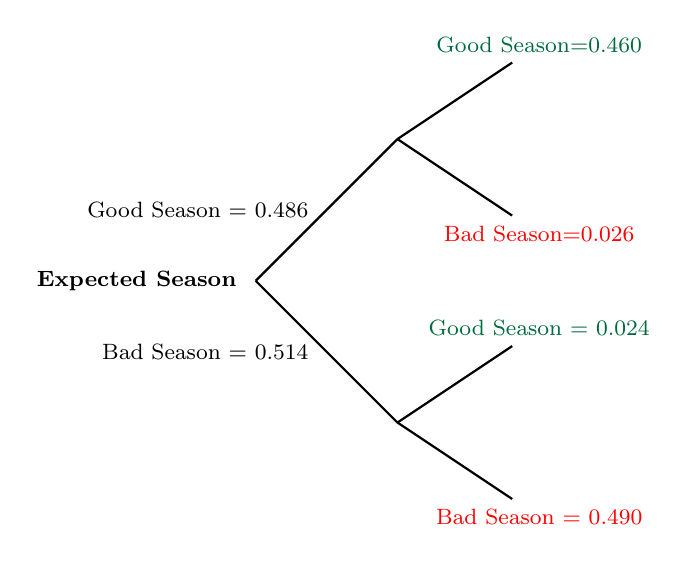
\begin{tikzpicture}[scale=0.6,thick,
    level/.style={level distance=3cm},
    level 2/.style={sibling distance=6cm},
    level 3/.style={sibling distance=4cm}
]
\coordinate
child[grow=right, level distance=0pt] {
        child  {
            child {
                node {{\footnotesize \textcolor{red}{Bad Season = 0.490}}}
                edge from parent 
            }
            child {
                node {{\footnotesize \textcolor{cadmiumgreen}{Good Season = 0.024}}}
                edge from parent
            }
            edge from parent
            node [left] {{\footnotesize Bad Season = 0.514 \ }}
        }
        child {
            child {
                node {{\footnotesize \textcolor{red}{Bad Season=0.026}}}
                edge from parent
            }
            child {
                node {{\footnotesize \textcolor{cadmiumgreen}{Good Season=0.460}}}
                edge from parent  
            }
            edge from parent 
            node [left] {{\footnotesize Good Season = 0.486 \ }}
        }
        node [left] {{\footnotesize \textbf{Expected Season\ \ }}}
    };
\end{tikzpicture}
\end{figure}
\end{frame}

\begin{frame}
\begin{center}
{\Large Appendix}
\end{center}
\end{frame}


\begin{frame}[label=NVSSseason2]
\frametitle{Season of Birth, Age and Education (Birth Order=2)}
\begin{table}[htbp]\centering
\def\sym#1{\ifmmode^{#1}\else\(^{#1}\)\fi}
\caption{Birth Quarter and Age (NVSS 2005-2013)}
\scalebox{0.8}{
\begin{tabular}{l*{4}{c}}
\toprule
                    &\multicolumn{1}{c}{(1)}   &\multicolumn{1}{c}{(2)}   &\multicolumn{1}{c}{(3)}   &\multicolumn{1}{c}{(4)}   \\
                    & Good Season   & Good Season   & Good Season   & Good Season   \\
\midrule
Aged 25-39          &       0.019***&       0.019***&       0.020***&       0.006   \\
                    &     [0.001]   &     [0.001]   &     [0.002]   &     [0.005]   \\
College Educ        &               &               &       0.010***&      -0.005   \\
                    &               &               &     [0.001]   &     [0.005]   \\
College$\times$ Aged 25-39&               &               &               &       0.015***\\
                    &               &               &               &     [0.005]   \\
Constant            &       0.497***&       0.497***&       0.488***&       0.501***\\
                    &     [0.001]   &     [0.001]   &     [0.002]   &     [0.005]   \\
\midrule
R-squared           &        0.00   &        0.00   &        0.00   &        0.00   \\
Observations        &     4871628   &     4871628   &     3613920   &     3613920   \\
Year FE&&Y&Y&Y\\ \bottomrule
\multicolumn{5}{p{12cm}}{\begin{footnotesize}Sample consists of all
first born children of US-born, white, non-hispanic mothers
\end{footnotesize}}\end{tabular}}\end{table}

\end{frame}

\begin{frame}[label=NVSSQuality2]
\frametitle{Birth Quality (Birth Order=2)}
\begin{table}[htbp]\centering
\def\sym#1{\ifmmode^{#1}\else\(^{#1}\)\fi}
\caption{Birth Quality by Age and Season (NVSS 2005-2013)}
\scalebox{0.68}{
\begin{tabular}{l*{7}{c}}
\toprule
                    &\multicolumn{1}{c}{(1)}   &\multicolumn{1}{c}{(2)}   &\multicolumn{1}{c}{(3)}   &\multicolumn{1}{c}{(4)}   &\multicolumn{1}{c}{(5)}   &\multicolumn{1}{c}{(6)}   &\multicolumn{1}{c}{(7)}   \\
                    &       APGAR   & Birthweight   &   Gestation   &         LBW   &   Premature   &        Twin   &        VLBW   \\
\midrule
Aged 25-39          &       0.043***&     130.718***&       0.598***&      -0.055***&      -0.064***&      -0.054***&      -0.010***\\
                    &     [0.004]   &     [2.581]   &     [0.011]   &     [0.001]   &     [0.001]   &     [0.001]   &     [0.000]   \\
Bad Season          &       0.002   &      -5.653   &      -0.011   &       0.004** &       0.002   &       0.001   &      -0.001*  \\
                    &     [0.005]   &     [3.585]   &     [0.015]   &     [0.002]   &     [0.002]   &     [0.001]   &     [0.001]   \\
Young$\times$ Bad S &      -0.005   &      -4.781   &      -0.014   &      -0.001   &       0.001   &       0.001   &       0.002***\\
                    &     [0.005]   &     [3.638]   &     [0.015]   &     [0.002]   &     [0.002]   &     [0.001]   &     [0.001]   \\
College Educ        &       0.045***&      77.112***&       0.181***&      -0.025***&      -0.021***&       0.010***&      -0.006***\\
                    &     [0.001]   &     [0.917]   &     [0.004]   &     [0.000]   &     [0.000]   &     [0.000]   &     [0.000]   \\
&&&&&&&\\
Constant            &       8.756***&    3121.397***&      38.034***&       0.150***&       0.194***&       1.075***&       0.028***\\
                    &     [0.004]   &     [2.775]   &     [0.012]   &     [0.001]   &     [0.001]   &     [0.001]   &     [0.001]   \\
\midrule
R-squared           &        0.00   &        0.00   &        0.00   &        0.00   &        0.00   &        0.00   &        0.00   \\
Observations        &     3551931   &     3603294   &     3610749   &     3613920   &     3613920   &     3613920   &     3613920   \\
\bottomrule
\multicolumn{8}{p{15cm}}{\begin{footnotesize}Sample consists of all
first born children of US-born, white, non-hispanic mothers
\end{footnotesize}}\end{tabular}}\end{table}

\end{frame}


\begin{frame}[label=NVSStwin]
\frametitle{Season of Birth, Age and Education (Twins)}
\input{./tables/NVSSBinaryTwin.tex}
\end{frame}

\begin{frame}[label=NVSSQualitytwin]
\frametitle{Birth Quality (Twins)}
\input{./tables/NVSSQualityTwin.tex}
\end{frame}

\begin{frame}[label=NVSSFD]
\frametitle{Season of Birth, Age and Education (Fetal Deaths)}
\input{./tables/NVSSBinaryFDeathsOnly.tex}
\end{frame}




\end{document}
%********************************************************************************



